% Provenance (never printed): see sources/outline_sources.md (Year 3:
% stereographic projection; fold and fault analysis; palaeostress; balanced
% cross-sections). Brief: sources/book5/BRIEFS.md, ch. 8. Nets, pi-diagram and
% fault-slip data from figdata/bachelor-3/stereonet.py (Varden data invented,
% from figdata/shared/region.py); Fry plot from figdata/bachelor-3/fry.py.
% Exercise and problem values in the Book 5 scratch calculator calc/ch08.py.
% No real-world numbers: no ledger rows.
\chapter{Analyse structurale}\label{ch:b3:structural-analysis}

Un géologue a mesuré deux cents plans de stratification sur les flancs d'un pli
trop vaste pour être vu d'un seul tenant~: sa charnière se trouve sous une forêt, ses flancs s'étendent sur
des kilomètres. Chaque mesure est un couple de nombres. Reportées sous forme de points sur un abaque circulaire,
les \omterm{def:b3:structural-analysis:stereo}{pôles} des plans s'alignent sur une seule courbe, un grand cercle, et
le \omterm{def:b3:structural-analysis:stereo}{pôle} de ce grand cercle est l'axe du pli, une droite que personne n'a
jamais vue. Ce chapitre construit l'abaque, la \omterm{def:b3:structural-analysis:stereo}{projection stéréographique}, et
l'utilise, avec les outils vectoriels qui le sous-tendent, pour trouver les axes de pli, mesurer la
déformation enregistrée par des objets déformés, retrouver la contrainte à l'origine d'un jeu de
failles, et restaurer une coupe déformée dans son état antérieur à la
déformation.

\begin{recall}
Les grands et petits cercles d'une sphère figurent dans le volume de première année, dans son chapitre
sur l'astronomie sphérique~; direction, pendage, sens du pendage, azimut et plongement dans ses
chapitres sur les cartes géologiques et les coupes~; la normale unitaire ascendante
d'un plan de sens de pendage $\alpha$ et de pendage $\delta$, $\vec n = (\sin\delta
\sin\alpha, \sin\delta\cos\alpha, \cos\delta)$ en composantes est, nord et haut
et la moyenne vectorielle d'un ensemble de mesures dans son premier chapitre sur
les méthodes de terrain et de laboratoire. Les éléments et les classes de plis, la ligne de charnière
d'un pli, parallèle à $\vec n_1\times\vec n_2$ et l'angle entre flancs
$\ang{180} - \arccos(\vec n_1\cdot\vec n_2)$, ainsi que la théorie d'Anderson
sur la rupture en faille, se trouvent dans son chapitre sur les failles, les plis et les fabriques~; la contrainte, les
contraintes principales, l'ellipse de déformation et le cisaillement simple, dans son chapitre sur
la contrainte, la déformation et la rhéologie~; le pitch d'un vecteur glissement (à partir de la direction,
\ang{-90} pour une faille normale, \ang{90} pour une faille inverse, 0 pour un jeu senestre et
\ang{180} pour un jeu dextre) et les axes P et T d'un mécanisme au foyer, dans son chapitre sur
la source sismique. La coupe équilibrée et le décollement figurent dans
le volume de deuxième année, dans son chapitre sur les Alpes. Les moindres carrés se trouvent dans
la \cref{sec:b3:seismology-imaging:inverse}~; les valeurs propres et les vecteurs propres
d'une matrice symétrique figurent dans les volumes de mathématiques.
\end{recall}

\section{La projection stéréographique}\label{sec:b3:structural-analysis:stereo}

Les données du géologue sont des orientations~: l'attitude d'un plan de stratification, d'une
faille, d'une foliation~; l'azimut et le plongement d'une linéation, d'une charnière de pli et d'une
direction de glissement. Chacune est une direction passant par un point, sans position. Pour
comparer des centaines d'entre elles, imaginons-les toutes ramenées au centre d'une sphère~:
une droite rencontre la moitié inférieure de la sphère en un point, un plan la coupe selon
un demi-grand cercle. Une carte de l'hémisphère inférieur montre alors les droites comme
points et les plans comme des courbes.

\begin{definition}[Projection stéréographique, canevas équiangle, projection équivalente, pôle]\label{def:b3:structural-analysis:stereo}
Soit une droite passant par le centre $O$ d'une sphère de rayon $R$ et coupant
l'hémisphère inférieur en $P$, sous l'angle $\theta = \ang{90} - p$ à partir du nadir, où
$p$ est le plongement de la droite et $t$ son azimut. La \emph{projection
stéréographique}\index{projection stéréographique} associe $P$ au point où la
droite menée du zénith à $P$ coupe le plan horizontal passant par
$O$~; ce point se trouve à la distance $r$ de $O$, dans l'azimut $t$. La
carte de l'hémisphère inférieur ainsi tracée, avec son quadrillage de grands et petits
cercles, est le \emph{canevas équiangle}\index{canevas équiangle} (ou
canevas de Wulff). La \emph{projection équivalente}\index{projection équivalente (de la sphère)}
envoie $P$ sur le point situé à la distance $r =
R\sqrt2\sin(\theta/2)$ dans l'azimut $t$~; son canevas est le canevas de Schmidt. Le
\emph{pôle}\index{pôle (à un plan)} d'un plan est sa droite normale, représentée comme
un point~: pour un plan de sens de pendage $\alpha$ et de pendage $\delta$, le pôle
a pour azimut $\alpha + \ang{180}$ et pour plongement $\ang{90} - \delta$.
\end{definition}

Les deux projections placent une verticale au centre et une horizontale sur
le cercle de rayon $R$, la primitive. Elles diffèrent par ce qu'elles conservent.

\begin{theorem}[Les deux projections]\label{thm:b3:structural-analysis:projections}
\begin{enumerate}[label=(\alph*)]
  \item La \omterm{def:b3:structural-analysis:stereo}{projection stéréographique} place $P$ en $r = R\tan(\theta/2)$. Elle
        est conforme~: en chaque point, elle dilate toutes les directions du même
        facteur, $1/(2\cos^2(\theta/2))$, de sorte qu'elle conserve les angles entre
        courbes.
  \item La \omterm{def:b3:structural-analysis:stereo}{projection équivalente} multiplie toute aire par le même facteur,
        $1/2$~: l'aire d'une région du canevas vaut la moitié de l'aire de la région
        de l'hémisphère qu'elle représente.
\end{enumerate}
\end{theorem}

\begin{proof}
(a) Dans le plan vertical passant par le zénith $Z$, le nadir et $P$
(première figure ci-dessous), l'arc du nadir à $P$
sous-tend l'angle $\theta$ au centre, donc l'angle inscrit
$\theta/2$ en $Z$, situé à la distance $R$ au-dessus de $O$~: $r =
R\tan(\theta/2)$. Un petit pas $R\,\mathrm d\theta$ sur la sphère vers le
nadir devient $\mathrm dr = R\,\mathrm d\theta/(2\cos^2(\theta/2))$ sur le
canevas. Le cercle des points situés à l'angle $\theta$ du nadir a
pour circonférence $2\pi R\sin\theta$ et devient un cercle de circonférence $2\pi
r$~; le rapport vaut $\tan(\theta/2)/\sin\theta = 1/(2\cos^2(\theta/2))$, le même
que le long du rayon. Une carte qui dilate également selon deux directions perpendiculaires
dilate de la même façon dans toutes les directions et conserve les angles.

(b) La calotte de la sphère comprise dans l'angle $\theta$ du nadir a pour aire
$2\pi R^2(1 - \cos\theta) = 4\pi R^2\sin^2(\theta/2)$~; son image est le disque
d'aire $\pi r^2 = 2\pi R^2\sin^2(\theta/2)$, moitié de celle-ci. Les deux aires sont
réparties uniformément en azimut, si bien que le secteur de la calotte compris entre deux azimuts
et son image gardent le rapport $1/2$, et il en va de même pour l'anneau compris entre deux valeurs
de $\theta$, différence de deux calottes. Toute région est une réunion de tels
petits secteurs annulaires.
\end{proof}

La \omterm{def:b3:structural-analysis:stereo}{projection stéréographique} transforme aussi tout cercle de la sphère, grand ou
petit, en un cercle ou une droite du canevas~; nous l'admettons. Elle rend le
\omterm{def:b3:structural-analysis:stereo}{canevas équiangle} facile à tracer au compas, et un petit cercle, le cône des
droites faisant un angle fixe avec un axe, conserve sa forme. La \omterm{def:b3:structural-analysis:stereo}{projection équivalente}
déforme les formes~: un petit cercle devient un ovale étiré
autour de la primitive. C'est la projection sur laquelle un nuage de \omterm{def:b3:structural-analysis:stereo}{pôles} peut être
dénombré, puisque des aires égales du canevas contiennent une part égale des
directions de l'hémisphère~; les géologues structuraux, et les sismologues pour leurs
mécanismes au foyer, l'utilisent pour leurs données.

\begin{omfigure}
\begin{tikzpicture}[scale=1.0, >=stealth]
% (a) equal-angle: theta = 60 deg, R = 2 cm; r = 2 tan 30 = 1.155
\begin{scope}
\draw[thick] (0,0) circle (2);
\draw (-2.5,0) -- (2.5,0) node[right, font=\scriptsize] {plan};
\fill (0,2) circle (1.5pt) node[above, font=\scriptsize] {zénith $Z$};
\fill (0,-2) circle (1.5pt) node[below, font=\scriptsize] {nadir};
\fill (0,0) circle (1.2pt) node[above left, font=\scriptsize] {$O$};
\draw[dashed] (0,2) -- (0,-2);
\draw[omDef, thick] (0,0) -- (1.732,-1);
\fill[omDef] (1.732,-1) circle (1.5pt) node[below right, font=\scriptsize] {$P$};
\draw[omThm] (0,2) -- (1.732,-1);
\fill[omThm] (1.155,0) circle (1.5pt);
\node[omThm, font=\scriptsize, above right] at (1.155,0) {$P'$};
\draw (0,-0.6) arc[start angle=-90, end angle=-30, radius=0.6];
\node[font=\scriptsize] at (0.38,-0.85) {$\theta$};
\draw (0,1.2) arc[start angle=-90, end angle=-60, radius=0.8];
\node[font=\scriptsize] at (0.25,0.95) {$\theta/2$};
\draw[<->] (0,0.25) -- (1.155,0.25);
\node[font=\scriptsize, above] at (0.58,0.25) {$r$};
\node[font=\small] at (0,-3.0) {(a) équiangle};
\end{scope}
% (b) equal-area: chord from nadir to P = 2R sin(theta/2) = 2
\begin{scope}[xshift=6.6cm]
\draw[thick] (0,0) circle (2);
\draw (-2.5,0) -- (2.5,0);
\draw (-2.5,-2) -- (2.5,-2) node[right, font=\scriptsize] {plan tangent};
\fill (0,-2) circle (1.5pt) node[below left, font=\scriptsize] {nadir};
\fill (0,0) circle (1.2pt) node[above left, font=\scriptsize] {$O$};
\draw[dashed] (0,2) -- (0,-2);
\draw[omDef, thick] (0,0) -- (1.732,-1);
\fill[omDef] (1.732,-1) circle (1.5pt) node[above right, font=\scriptsize] {$P$};
\draw[omThm] (0,-2) -- (1.732,-1);
\draw[omThm, dashed] (1.732,-1) arc[start angle=30, end angle=0, radius=2];
\fill[omThm] (2,-2) circle (1.5pt);
\node[omThm, font=\scriptsize, below] at (2,-2.05) {$2R\sin(\theta/2)$};
\draw (0,-0.6) arc[start angle=-90, end angle=-30, radius=0.6];
\node[font=\scriptsize] at (0.38,-0.85) {$\theta$};
\node[font=\small] at (0,-3.0) {(b) équivalente};
\end{scope}
\end{tikzpicture}

\par\smallskip{\small Les deux projections, dans le plan vertical passant par la
droite $OP$. (a) La \omterm{def:b3:structural-analysis:stereo}{projection stéréographique} envoie $P$ en $P'$, où la droite
issue du zénith coupe le plan horizontal~: l'angle en $Z$ vaut
$\theta/2$, donc $r = R\tan(\theta/2)$. (b) La \omterm{def:b3:structural-analysis:stereo}{projection équivalente} porte
$P$, autour du nadir, sur le plan tangent à la distance $2R\sin(\theta/2)$
de la corde~; le canevas est ensuite réduit d'un facteur $1/\sqrt2$ afin que les
droites horizontales tombent sur une primitive de rayon $R$.}\label{fig:b3:structural-analysis:geometry}
\end{omfigure}

\begin{omfigure}
\begin{tikzpicture}
\begin{groupplot}[group style={group size=2 by 1, horizontal sep=0.8cm},
  width=0.5\linewidth, height=0.5\linewidth, axis equal image, hide axis,
  xmin=-1.15, xmax=1.15, ymin=-1.15, ymax=1.15, unbounded coords=jump,
  title style={font=\small}]
\nextgroupplot[title={(a) canevas équiangle (Wulff)}]
% computed in figdata/bachelor-3/stereonet.py
\addplot[gray!75, very thin] table[x=x, y=y] {figdata/out/bachelor-3-stereonet-wulff.dat};
\addplot[gray!75, very thin] coordinates {(-1,0) (1,0)};
\addplot[black, thick, domain=0:360, samples=181] ({cos(x)}, {sin(x)});
\node[font=\scriptsize, above] at (axis cs:0,1.0) {N};
\nextgroupplot[title={(b) canevas équivalent (Schmidt)}]
\addplot[gray!75, very thin] table[x=x, y=y] {figdata/out/bachelor-3-stereonet-schmidt.dat};
\addplot[gray!75, very thin] coordinates {(-1,0) (1,0)};
\addplot[black, thick, domain=0:360, samples=181] ({cos(x)}, {sin(x)});
\node[font=\scriptsize, above] at (axis cs:0,1.0) {N};
\end{groupplot}
\end{tikzpicture}

\par\smallskip{\small Les deux canevas, construits à partir des formules du théorème
ci-dessus~: grands cercles des plans de direction nord--sud et de pendage
\ang{10} vers l'est et vers l'ouest, et petits cercles tous les \ang{10} autour de
l'axe nord--sud. Sur le \omterm{def:b3:structural-analysis:stereo}{canevas équiangle} les petits cercles sont des cercles~; sur
le canevas équivalent ce sont des ovales, mais des aires égales contiennent des
parts égales de directions.}\label{fig:b3:structural-analysis:nets}
\end{omfigure}

\paragraph{Plans, droites et angles.}
Un plan de sens du pendage $\alpha$ et de pendage $\delta$ coupe l'hémisphère
inférieur selon un demi-grand cercle. Ses extrémités se trouvent sur la primitive
aux deux bouts de la direction~; son milieu est la ligne de plus grande pente, qui
plonge de $\delta$ vers $\alpha$~; et son \omterm{def:b3:structural-analysis:stereo}{pôle} est situé à \ang{90} de chacun de
ses points, dans l'azimut $\alpha + \ang{180}$. Une droite du plan est un point du grand
cercle. Pour reporter des données, on pose sur le canevas une feuille transparente
que l'on fait tourner autour du centre jusqu'à ce que la direction des données se place
le long du diamètre nord--sud du canevas~; on trace alors le grand cercle du bon pendage, puis on remet la feuille
en place. L'angle entre deux droites se mesure le long du grand cercle qui passe
par les deux points, en comptant les divisions des petits cercles qu'il traverse,
après avoir fait tourner la feuille jusqu'à ce que les deux points se trouvent sur un même grand cercle du canevas.
L'angle entre deux plans est l'angle entre leurs \omterm{def:b3:structural-analysis:stereo}{pôles}, ou son supplémentaire.
Un ordinateur fait de même avec des vecteurs~: l'angle entre deux droites de vecteurs
unitaires $\vec u$ et $\vec v$ vaut $\arccos|\vec u\cdot\vec v|$.

\begin{method}[Rotation des données autour d'un axe]\label{met:b3:structural-analysis:rotation}
Pour défaire un basculement, par exemple pour ramener une couche à l'horizontale
avec les linéations qu'elle porte, ou pour restaurer une direction paléomagnétique
mesurée dans des strates basculées (\cref{ch:b3:palaeomagnetism})~:
\begin{enumerate}
  \item Choisir l'axe de rotation~: pour une couche basculée, sa ligne de direction,
        horizontale~; l'angle est le pendage, dans le sens qui relève la couche.
  \item Sur le canevas, faire tourner la feuille jusqu'à ce que l'axe se place le
        long du diamètre nord--sud, où les petits cercles sont les cônes qui
        l'entourent.
  \item Déplacer chaque point le long de son petit cercle de l'angle de rotation,
        compté sur les grands cercles. Un point qui sortirait de l'hémisphère
        inférieur réapparaît à l'autre extrémité de son petit cercle, dans
        l'azimut opposé.
  \item Remettre la feuille en place. Avec des vecteurs, la rotation de $\vec v$
        d'un angle $\omega$ autour du vecteur unitaire $\vec k$ vaut $\vec v' = \vec v
        \cos\omega + (\vec k\times\vec v)\sin\omega + \vec k(\vec k\cdot\vec
        v)(1 - \cos\omega)$.
\end{enumerate}
\end{method}

\section{Analyse des plis}\label{sec:b3:structural-analysis:folds}

Un pli cylindrique est engendré par une droite, l'axe du pli, déplacée
parallèlement à elle-même. Tout plan tangent à la surface plissée contient
l'axe, donc toute normale à la surface est perpendiculaire à cet axe~: tous les
\omterm{def:b3:structural-analysis:stereo}{pôles} se situent sur le grand cercle du plan perpendiculaire à l'axe.

\begin{definition}[Diagramme pi, axe bêta]\label{def:b3:structural-analysis:pi}
Le \emph{diagramme pi}\index{diagramme pi} d'un pli est le tracé des \omterm{def:b3:structural-analysis:stereo}{pôles} des
plans mesurés sur sa surface plissée. Pour un pli cylindrique, ils se situent sur
un grand cercle, la $\pi$-ceinture~; le \omterm{def:b3:structural-analysis:stereo}{pôle} de la ceinture est le
\emph{axe bêta}\index{axe bêta}, l'estimation de l'axe du pli donnée par les
mesures.
\end{definition}

Avec deux flancs seulement, l'\omterm{def:b3:structural-analysis:pi}{axe bêta} est le produit vectoriel de leurs normales, comme
le volume de première année l'a montré pour la ligne de charnière. Avec deux cents
mesures dispersées, un ajustement optimal est nécessaire. Le vecteur moyen, qui a servi pour les
mesures d'un seul plan, ne convient pas~: les \omterm{def:b3:structural-analysis:stereo}{pôles} d'une ceinture se répartissent dans toutes les directions le long de celle-ci, et
leur moyenne dit peu de chose du cercle sur lequel ils se trouvent.

\begin{definition}[Tenseur d'orientation]\label{def:b3:structural-analysis:orientation-tensor}
Le \emph{tenseur d'orientation}\index{tenseur d'orientation} de $N$ vecteurs unitaires
$\vec p_1, \dots, \vec p_N$ est la matrice symétrique
\[
  T = \frac1N\sum_{i=1}^N \vec p_i\,\vec p_i^{\mathsf T},
  \qquad T_{jk} = \frac1N\sum_i p_{ij}\,p_{ik} .
\]
Il ne change pas lorsqu'un vecteur est remplacé par son opposé, il convient donc
aux axes et aux \omterm{def:b3:structural-analysis:stereo}{pôles}, qui n'ont pas de sens. Ses valeurs propres $\lambda_1 \ge \lambda_2
\ge \lambda_3 \ge 0$ ont pour somme sa trace, $1$.
\end{definition}

\begin{theorem}[Amas et ceinture à partir du tenseur d'orientation]\label{thm:b3:structural-analysis:tensor}
Pour tout vecteur unitaire $\vec u$,
\[
  \frac1N\sum_{i=1}^N (\vec p_i\cdot\vec u)^2 = \vec u^{\mathsf T}T\,\vec u ,
\]
qui atteint sa plus petite valeur, $\lambda_3$, lorsque $\vec u$ est le vecteur propre
$\vec e_3$ associé à la plus petite valeur propre, et sa plus grande, $\lambda_1$, le long du
vecteur propre $\vec e_1$. Comme $\vec p_i\cdot\vec u$ est le sinus de l'angle
entre $\vec p_i$ et le plan perpendiculaire à $\vec u$, le grand cercle
perpendiculaire à $\vec e_3$ est la ceinture qui minimise la somme des carrés des
sinus des distances des \omterm{def:b3:structural-analysis:stereo}{pôles} à ce cercle, et $\sqrt{\lambda_3}$ est leur
sinus quadratique moyen. L'axe $\vec e_1$ est la droite la plus proche des vecteurs,
l'axe moyen d'un amas.
\end{theorem}

\begin{proof}
$(\vec p_i\cdot\vec u)^2 = \vec u^{\mathsf T}\vec p_i\,\vec p_i^{\mathsf T}\vec
u$~; on moyenne sur $i$. La matrice $T$ est symétrique, donc elle admet une base orthonormée
de vecteurs propres, dans laquelle $\vec u = \sum_k u_k\vec e_k$ avec $\sum_k
u_k^2 = 1$ et $\vec u^{\mathsf T}T\vec u = \sum_k\lambda_k u_k^2$. Il s'agit d'une
moyenne pondérée des valeurs propres, de poids $u_k^2$ dont la somme vaut 1~: elle
se situe entre $\lambda_3$ et $\lambda_1$ et les atteint pour $\vec u = \vec
e_3$ et $\vec e_1$.
\end{proof}

Les valeurs propres décrivent la forme des données. Un amas a $\lambda_1$ proche de
1 et les deux autres petites~; une ceinture a $\lambda_3$ proche de 0, les \omterm{def:b3:structural-analysis:stereo}{pôles} étant
répartis le long du cercle de sorte que $\lambda_1$ et $\lambda_2$ se partagent le reste~;
des vecteurs dispersés uniformément donnent trois valeurs propres proches de $1/3$. Un pli est
cylindrique, à la précision des mesures près, lorsque $\sqrt{\lambda_3}$ est
non supérieur à la dispersion des mesures répétées d'un même plan. Un pli conique,
ou deux générations de plis, écartent les \omterm{def:b3:structural-analysis:stereo}{pôles} de tout grand cercle
et augmentent $\lambda_3$.

La figure ci-dessous représente douze mesures prises sur les deux flancs de l'anticlinal
de Varden, pli fictif de la série (\cref{pb:b3:structural-analysis:1}
calcule son axe). Les \omterm{def:b3:structural-analysis:stereo}{pôles} des flancs peu inclinés se regroupent près du centre du
canevas en deux groupes, qui définissent ensemble une ceinture orientée presque
est-ouest~; l'\omterm{def:b3:structural-analysis:pi}{axe bêta} se situe sur la primitive, presque plein nord. Les plans moyens
des deux flancs, tracés comme grands cercles, se coupent au même point~:
l'\omterm{def:b3:structural-analysis:pi}{axe bêta} est la droite commune à tous les flancs.

\begin{omfigure}
\begin{tikzpicture}
\begin{groupplot}[group style={group size=2 by 1, horizontal sep=1.0cm},
  width=0.5\linewidth, height=0.5\linewidth, axis equal image,
  unbounded coords=jump, title style={font=\small}]
\nextgroupplot[hide axis, xmin=-1.15, xmax=1.15, ymin=-1.15, ymax=1.15,
  title={(a) l'hémisphère inférieur}]
% computed in figdata/bachelor-3/stereonet.py (Varden readings invented)
\addplot[gray!35, very thin] table[x=x, y=y] {figdata/out/bachelor-3-stereonet-schmidt.dat};
\addplot[black, thick, domain=0:360, samples=181] ({cos(x)}, {sin(x)});
\addplot[gray, densely dashed] table[x=x, y=y] {figdata/out/bachelor-3-stereonet-limbs.dat};
\addplot[omDef, thick] table[x=x, y=y] {figdata/out/bachelor-3-stereonet-girdle.dat};
\addplot[only marks, mark=*, mark size=1.2pt] table[x=x, y=y] {figdata/out/bachelor-3-stereonet-poles.dat};
\addplot[only marks, mark=triangle*, mark size=3pt, omThm] table[x=x, y=y] {figdata/out/bachelor-3-stereonet-beta.dat};
\node[font=\scriptsize, above] at (axis cs:0,1.02) {N};
\node[omThm, font=\scriptsize, right] at (axis cs:0.06,0.88) {$\beta$};
\draw[gray] (axis cs:-0.3,-0.3) rectangle (axis cs:0.3,0.3);
\nextgroupplot[xmin=-0.3, xmax=0.3, ymin=-0.3, ymax=0.3, title={(b) le centre, agrandi},
  xtick=\empty, ytick=\empty]
\addplot[gray!35, very thin] table[x=x, y=y] {figdata/out/bachelor-3-stereonet-schmidt.dat};
\addplot[omDef, thick] table[x=x, y=y] {figdata/out/bachelor-3-stereonet-girdle.dat};
\addplot[only marks, mark=*, mark size=1.5pt] table[x=x, y=y] {figdata/out/bachelor-3-stereonet-poles.dat};
\node[font=\scriptsize, align=center] at (axis cs:0.16,0.09) {pôles du\\ flanc ouest};
\node[font=\scriptsize, align=center] at (axis cs:-0.16,0.09) {pôles du\\ flanc est};
\node[omDef, font=\scriptsize] at (axis cs:0.17,-0.06) {$\pi$-ceinture};
\end{groupplot}
\end{tikzpicture}

\par\smallskip{\small \omterm{def:b3:structural-analysis:pi}{Diagramme pi} de l'anticlinal de Varden sur le canevas
équivalent, hémisphère inférieur~: les \omterm{def:b3:structural-analysis:stereo}{pôles} des douze mesures de stratification (points),
la ceinture de meilleur ajustement issue du \omterm{def:b3:structural-analysis:orientation-tensor}{tenseur d'orientation} (en bleu), les grands cercles des
deux flancs moyens (tiretés) et l'\omterm{def:b3:structural-analysis:pi}{axe bêta} (triangle), où se rejoignent les trois grands
cercles. Un banc à pendage est a son \omterm{def:b3:structural-analysis:stereo}{pôle} à l'ouest du
centre.}\label{fig:b3:structural-analysis:pi}
\end{omfigure}

\section{Analyse de la déformation finie}\label{sec:b3:structural-analysis:strain}

Une roche déformée enregistre sa déformation lorsqu'elle contient des objets dont la forme
initiale, ou la disposition initiale, est connue~: ooïdes arrondis et taches de réduction,
fossiles de symétrie connue, galets, ou simplement les centres de grains
qui étaient autrefois régulièrement espacés.

\begin{definition}[Analyse de la déformation finie, méthode de Fry]\label{def:b3:structural-analysis:strain-analysis}
L'\emph{analyse de la déformation finie}\index{analyse de la déformation finie} est la mesure
de l'ellipse de déformation, ou de l'ellipsoïde, qu'a subie une roche, à partir des
formes, des orientations ou des espacements d'objets dont l'état avant la
déformation est connu. Dans la \emph{méthode de Fry}\index{méthode de Fry}, on trace
le vecteur qui joint le centre de chaque objet au centre de chacun des autres, depuis
une origine commune~; lorsque les centres étaient répartis avec un espacement minimal et sans
direction privilégiée, la région vide autour de l'origine est une ellipse de la forme et
de l'orientation de l'ellipse de déformation.
\end{definition}

\begin{proposition}[Le vide de Fry]\label{prop:b3:structural-analysis:fry}
Si une déformation homogène transforme tout vecteur $\vec d$ en $F\vec d$, et si aucun couple
de centres n'était plus proche que $d_0$ avant la déformation, alors, après celle-ci, la région
autour de l'origine du diagramme de Fry, qui est vide de points, contient
l'ellipse $\{F\vec d : |\vec d| < d_0\}$, de demi-axes $S_1d_0$ et $S_2d_0$ selon les
directions principales de la déformation.
\end{proposition}

\begin{proof}
Une déformation homogène déplace chaque point par la même application linéaire, plus une
translation, de sorte que la différence de deux centres devient $F\vec d$. Avant la
déformation, aucune différence ne se trouvait dans le disque de rayon $d_0$~; après,
aucune ne se trouve dans son image, qui est l'ellipse de déformation du volume de première année, dilatée d'un facteur $d_0$.
\end{proof}

En pratique, les centres ne sont pas tous à l'espacement minimal, et le vide se lit
comme le bord intérieur de l'anneau le plus dense de points~; son rapport donne une estimation
légèrement faible du rapport de déformation $R_s = S_1/S_2$. La figure ci-dessous réalise le test
sur une lame mince inventée, déformée jusqu'à $R_s = 2$, avec le grand axe
à \ang{30} de l'horizontale~: l'ellipse ajustée au bord du vide donne
$R_s = 1.9$ et \ang{30}. Lorsque les objets eux-mêmes sont mesurés, les objets initialement
ronds deviennent exactement des ellipses de rapport d'axes $R_s$~; les objets initialement
elliptiques, d'orientations quelconques, finissent avec des rapports $R_f$ dispersés
autour de $R_s$, les plus grands lorsque leurs grands axes étaient initialement parallèles à
la direction d'étirement, et leurs orientations finales $\varphi$ se regroupent autour
de celle-ci. Le graphe de $R_f$ en fonction de $\varphi$, lu à l'aide de tables ou d'un ordinateur,
sépare la déformation des formes initiales.

\begin{omfigure}
\begin{tikzpicture}
\begin{groupplot}[group style={group size=2 by 1, horizontal sep=1.2cm},
  width=0.5\linewidth, height=0.5\linewidth, axis equal image,
  title style={font=\small}, tick label style={font=\scriptsize}]
\nextgroupplot[xmin=-10, xmax=10, ymin=-10, ymax=10, title={(a) centres de grains après la déformation}]
% computed in figdata/bachelor-3/fry.py (invented population)
\addplot[only marks, mark=o, mark size=1.6pt, black] table[x=x, y=y] {figdata/out/bachelor-3-fry-points.dat};
\nextgroupplot[xmin=-2.6, xmax=2.6, ymin=-2.6, ymax=2.6, title={(b) diagramme de Fry}]
\addplot[only marks, mark=*, mark size=0.5pt, black] table[x=x, y=y] {figdata/out/bachelor-3-fry-fry.dat};
\addplot[omThm, thick] table[x=x, y=y] {figdata/out/bachelor-3-fry-fit.dat};
\end{groupplot}
\end{tikzpicture}

\par\smallskip{\small La \omterm{def:b3:structural-analysis:strain-analysis}{méthode de Fry} sur une population inventée de centres de grains
disposés avec un espacement minimal de 1, puis déformés jusqu'à $R_s = 2$,
grand axe à \ang{30} dans le sens antihoraire de l'horizontale, surface conservée. (a) Les
centres, dans lesquels l'œil distingue à peine la déformation. (b) Les vecteurs entre toutes les
paires de centres plus proches que 2.6~: le centre vide est l'ellipse de déformation. L'ellipse
rouge est ajustée au point le plus proche dans chacun des 36 secteurs~: rapport 1.9,
grand axe à \ang{30}.}\label{fig:b3:structural-analysis:fry}
\end{omfigure}

En trois dimensions, l'ellipsoïde de déformation possède les étirements principaux $X \ge Y
\ge Z$. Sa forme se place sur le diagramme de Flinn, avec $a = X/Y$ en fonction de $b =
Y/Z$ et le paramètre
\[
  k = \frac{a - 1}{b - 1} .
\]
Sur la droite $k = 1$, qui correspond à la déformation plane à volume constant ($Y = 1$,
$X = 1/Z$, donc $a = b$), l'ellipsoïde n'est ni en cigare ni en crêpe. Au-dessus,
$k > 1$, l'ellipsoïde est allongé, étiré dans une direction par une
constriction~: les roches déformées de cette façon développent une forte linéation. En dessous, $k < 1$,
il est aplati, et la roche développe une forte foliation.

\begin{omfigure}
\begin{tikzpicture}[scale=1.0, >=stealth]
\draw[->] (0,0) -- (5.4,0) node[right, font=\scriptsize] {$b = Y/Z$};
\draw[->] (0,0) -- (0,4.6) node[above, font=\scriptsize] {$a = X/Y$};
\foreach \v/\l in {0/1, 1.5/2, 3/3, 4.5/4} {
  \draw (\v,0) -- (\v,-0.08) node[below, font=\scriptsize] {\l};
  \draw (0,\v) -- (-0.08,\v) node[left, font=\scriptsize] {\l};
}
\draw[omDef, thick] (0,0) -- (4.5,4.5) node[right, font=\scriptsize, align=left] {$k = 1$\\ déformation plane};
\node[font=\scriptsize, align=center] at (1.3,3.6) {constriction\\ $k > 1$, allongé};
\node[font=\scriptsize, align=center] at (4.3,1.1) {aplatissement\\ $k < 1$, aplati};
% shapes
\draw[fill=omLithLime] (0.9,2.75) ellipse (0.55 and 0.12);
\draw[fill=omLithLime] (4.3,2.1) ellipse (0.45 and 0.22);
\end{tikzpicture}

\par\smallskip{\small Diagramme de Flinn des ellipsoïdes de déformation. L'état non déformé
est à l'origine, $a = b = 1$~; les ellipsoïdes en cigare de constriction
se rangent vers l'axe vertical, les crêpes d'aplatissement vers
l'axe horizontal.}\label{fig:b3:structural-analysis:flinn}
\end{omfigure}

\section{Paléocontrainte}\label{sec:b3:structural-analysis:palaeostress}

La théorie d'Anderson indique sur quels plans se forment de nouvelles failles, et qu'elles glissent
perpendiculairement à $\sigma_2$. La plupart des failles, cependant, sont d'anciennes zones de
faiblesse réactivées dans un champ de contrainte qu'elles n'ont pas choisi, et elles glissent
de façon oblique. Leurs directions de glissement, lues sur les stries des
surfaces de faille, enregistrent encore la contrainte, à condition que chaque faille glisse dans le sens où la
contrainte la pousse.

\begin{definition}[Paléocontrainte, hypothèse de Wallace--Bott, rapport de contraintes, inversion des stries de faille]\label{def:b3:structural-analysis:palaeostress}
La \emph{paléocontrainte}\index{paléocontrainte} est l'état de contrainte qui a agi
dans une roche par le passé, dans la mesure où l'on peut le déduire des structures qu'elle a laissées~:
en pratique, les directions des contraintes principales et le
\emph{rapport de contraintes}\index{rapport de contraintes}
\[
  \Phi = \frac{\sigma_2 - \sigma_3}{\sigma_1 - \sigma_3}, \qquad 0 \le \Phi
  \le 1 .
\]
L'\emph{hypothèse de Wallace--Bott}\index{hypothèse de Wallace--Bott} postule
qu'une faille glisse parallèlement à la contrainte de cisaillement projetée sur son plan par une
contrainte uniforme, chaque faille indépendamment. L'\emph{inversion des stries de
faille}\index{inversion des stries de faille} est la recherche des directions principales
et du rapport de contraintes dont les directions de glissement prédites ajustent au mieux un ensemble de
failles et de stries mesurées.
\end{definition}

\begin{theorem}[Direction de glissement sur un plan]\label{thm:b3:structural-analysis:wallace-bott}
Soit $S$ le tenseur des contraintes, les compressions étant comptées positivement, et $\vec n$ la
normale unitaire ascendante d'une faille. On pose
\[
  \vec\tau = S\vec n - (\vec n\cdot S\vec n)\,\vec n .
\]
Sous l'\omterm{def:b3:structural-analysis:palaeostress}{hypothèse de Wallace--Bott}, le toit glisse par rapport au
mur le long de $-\vec\tau$, la traction de cisaillement qu'il exerce sur le
mur. De plus~:
\begin{enumerate}[label=(\alph*)]
  \item la direction de $\vec\tau$ est inchangée lorsque $S$ est remplacé par $aS +
        bI$ avec $a > 0$~; elle ne dépend donc que des directions principales et de $\Phi$, et le
        tenseur réduit $S' =
        \mathrm{diag}(1, \Phi, 0)$ dans le repère principal $(\vec e_1, \vec
        e_2, \vec e_3)$ prédit le même glissement que $S$~;
  \item si $\vec n$ est perpendiculaire à une direction principale,
        le glissement l'est aussi~;
  \item avec $n_k = \vec n\cdot\vec e_k$, la direction est celle de $\vec\tau'
        = \vec\tau_0 + \Phi\,\vec\tau_1$, linéaire en $\Phi$, où $\vec\tau_0
        = n_1(\vec e_1 - n_1\vec n)$ et $\vec\tau_1 = n_2(\vec e_2 - n_2\vec
        n)$.
\end{enumerate}
\end{theorem}

\begin{proof}
Les compressions étant comptées positivement, le toit pousse sur le mur, à travers le
plan de normale $\vec n$ pointant vers le toit, avec la
traction $-S\vec n$~; sa composante le long du plan est $-\vec\tau$. Lorsque la
faille glisse, le toit se déplace dans le sens où il entraîne le mur, le long de
$-\vec\tau$. (Vérification~: avec $\sigma_1$ vertical, $S = \sigma_1\vec e_z\vec
e_z^{\mathsf T}$ et $-\vec\tau = -\sigma_1\cos\delta\,(\vec e_z -
\cos\delta\,\vec n)$ pointe vers le bas du pendage~: il s'agit d'une faille normale.)
(a)~: $(aS + bI)\vec n - (\vec n\cdot(aS + bI)\vec n)\vec n = a\vec\tau + b(\vec
n - \vec n) = a\vec\tau$. En écrivant $\sigma_k = \sigma_3 + (\sigma_1 -
\sigma_3)s_k$ avec $s = (1, \Phi, 0)$, on obtient $S = \sigma_3 I + (\sigma_1 -
\sigma_3)S'$.
(b) $S\vec n = \sum_k\sigma_kn_k\vec e_k$~; si $n_j = 0$, ni $S\vec n$
ni $\vec n$ n'ont de composante selon $\vec e_j$, et il en va de même pour $\vec\tau$.
(c) $S'\vec n = n_1\vec e_1 + \Phi n_2\vec e_2$ et $\vec n\cdot S'\vec n =
n_1^2 + \Phi n_2^2$~; on regroupe les termes avec et sans $\Phi$.
\end{proof}

La partie (b) est le cas d'Anderson~: une faille qui contient $\sigma_2$ glisse
perpendiculairement à lui, quel que soit $\Phi$, de sorte qu'elle ne dit rien du
\omterm{def:b3:structural-analysis:palaeostress}{rapport de contraintes}. La partie (c) transforme un glissement mesuré en $\Phi$. Soit $\vec u$ le
vecteur glissement unitaire du toit, déduit du pitch, et $\vec w = \vec n\times\vec
u$ la direction du plan perpendiculaire à celui-ci. Le glissement prédit est
parallèle à $\vec u$ lorsque $(\vec\tau_0 + \Phi\vec\tau_1)\cdot\vec w = 0$, et
comme $\vec n\cdot\vec w = 0$,
\[
  \Phi = -\frac{n_1\,(\vec e_1\cdot\vec w)}{n_2\,(\vec e_2\cdot\vec w)} ,
\]
à condition que le glissement prédit pointe alors selon $+\vec u$ et non $-\vec u$.

Lorsque les directions principales ne sont pas connues, chaque faille fournit une équation,
l'angle de son glissement dans son plan, pour quatre inconnues~: trois angles qui
orientent les axes principaux, et $\Phi$. Quatre failles d'attitudes différentes constituent
le minimum, et quelques dizaines sont courantes. L'inversion minimise la somme des
carrés des écarts angulaires entre les glissements mesurés et prédits, par moindres carrés
sur une grille ou par itération comme dans la \cref{sec:b3:seismology-imaging:inverse}.
Les failles qui ne s'ajustent pas forment une seconde population, peut-être d'un autre âge.

La figure ci-dessous présente cinq failles des monts Varden~: la faille normale principale
et quatre plus petites, toutes à glissement normal. Une recherche sur grille portant sur $\Phi$ et
l'azimut de $\sigma_3$, avec $\sigma_1$ vertical, ajuste les cinq failles à moins d'un quart
de degré près, avec $\sigma_3$ horizontal vers \ang{120}.

\begin{omfigure}
\begin{tikzpicture}
\begin{axis}[width=0.56\linewidth, height=0.56\linewidth, axis equal image,
  hide axis, xmin=-1.15, xmax=1.15, ymin=-1.15, ymax=1.15, unbounded coords=jump]
% computed in figdata/bachelor-3/stereonet.py (Varden faults invented)
\addplot[gray!35, very thin] table[x=x, y=y] {figdata/out/bachelor-3-stereonet-schmidt.dat};
\addplot[black, thick, domain=0:360, samples=181] ({cos(x)}, {sin(x)});
\addplot[omDef, thick] table[x=x, y=y] {figdata/out/bachelor-3-stereonet-faults.dat};
\addplot[only marks, mark=*, mark size=1.8pt, omDef] table[x=x, y=y] {figdata/out/bachelor-3-stereonet-slips.dat};
\addplot[only marks, mark=square*, mark size=2.6pt, omThm] table[x=x, y=y] {figdata/out/bachelor-3-stereonet-s1.dat};
\addplot[only marks, mark=diamond*, mark size=3pt, omProp] table[x=x, y=y] {figdata/out/bachelor-3-stereonet-s2.dat};
\addplot[only marks, mark=triangle*, mark size=3pt, omMeth] table[x=x, y=y] {figdata/out/bachelor-3-stereonet-s3.dat};
\node[font=\scriptsize, above] at (axis cs:0,1.02) {N};
\node[omThm, font=\scriptsize, above left] at (axis cs:0,0) {$\sigma_1$};
\node[omProp, font=\scriptsize, above right] at (axis cs:0.5,0.87) {$\sigma_2$};
\node[omMeth, font=\scriptsize, below right] at (axis cs:0.87,-0.5) {$\sigma_3$};
\end{axis}
\end{tikzpicture}

\par\smallskip{\small Données de stries des monts Varden sur le
canevas équivalent, hémisphère inférieur~: cinq plans de faille (grands cercles) avec
la direction de glissement de chaque toit (points), et les contraintes principales de la
meilleure contrainte ajustée~: $\sigma_1$ vertical (carré), $\sigma_2$ et $\sigma_3$
horizontaux (losanges et triangles, aux deux extrémités de chaque axe). La
faille principale, à \ang{60} de pendage vers \ang{120}, contient $\sigma_2$ et glisse
droit selon son pendage~; les autres glissent
obliquement.}\label{fig:b3:structural-analysis:faults}
\end{omfigure}

Les axes P et T du volume de première année ne sont pas les contraintes principales. Ils
sont construits à partir du plan de faille et du seul glissement, à \ang{45} du plan, dans
le plan qui contient le glissement et la normale~; une faille nouvelle, dans une roche d'angle
de frottement voisin de \ang{30}, fait environ \ang{30} avec $\sigma_1$, et une faille réactivée
fait un angle quelconque. Un seul mécanisme donne les axes P et T~; seules de nombreuses
failles d'attitudes différentes, inversées ensemble, donnent la contrainte. L'hypothèse
elle-même a des limites~: la contrainte peut varier d'une faille à l'autre, des blocs peuvent
tourner, et des failles qui se rencontrent se gênent dans leur glissement.

\section{Restauration d'une coupe}\label{sec:b3:structural-analysis:restoration}

Une coupe est une interprétation~: entre la surface et les forages, le géologue
dessine ce qui est vraisemblable. Le volume de deuxième année, dans son chapitre sur les
Alpes, appelle coupe équilibrée une coupe qui peut être ramenée à un état non déformé
en conservant les longueurs des couches et les aires des unités, les plis et les
chevauchements s'enracinant sur un décollement. La \omterm{def:b3:deformation-mechanisms:recrystallisation}{restauration} en est le test.

\begin{definition}[Restauration de coupe, ligne de référence, méthode des kink-bands]\label{def:b3:structural-analysis:restoration}
\emph{restauration de coupe}\index{restauration de coupe} défait, sur une coupe dessinée
parallèlement à la direction du transport tectonique, la déformation qu'elle montre,
événement par événement et dans l'ordre inverse, en conservant les longueurs des couches
et les aires des unités dans le plan de la coupe.
Une \emph{ligne de référence}\index{ligne de référence} est une ligne traversant les couches, placée là où elles
n'ont pas glissé l'une sur l'autre (dans l'avant-pays non déformé, ou sur la surface axiale
d'un pli symétrique), que l'on prend perpendiculaire aux couches
dans la coupe restaurée~; les longueurs sont mesurées à partir d'elle. Dans la
\emph{méthode des kink-bands}\index{méthode des kink-bands} les plis sont dessinés en flancs droits
d'épaisseur de couche constante, reliés par des charnières vives, dont les surfaces axiales
bissectent l'angle entre les flancs~; chaque couche est alors une ligne brisée, dont
la longueur est la somme de ses segments droits.
\end{definition}

Une couche pliée en flancs droits, de pendage $\delta$ dans un sens ou dans l'autre, sur la
distance horizontale $L$, a pour longueur $L/\cos\delta$~: son raccourcissement est
$S = L(1/\cos\delta - 1)$, la variation relative de longueur étant $\cos\delta - 1$.
Les aires fournissent l'autre moitié de l'équilibre.

\begin{proposition}[Profondeur du décollement]\label{prop:b3:structural-analysis:detachment}
Soit une couche située à la hauteur $h$ au-dessus d'un décollement horizontal, raccourcie de $S$
dans le plan d'une coupe, et que la roche comprise entre elle et le décollement
conserve son aire, sans matière franchissant les extrémités de la coupe. Alors l'aire
$A$ dont la couche plissée dépasse son niveau initial vérifie
\[
  A = S\,h , \qquad\text{d'où}\qquad h = \frac AS .
\]
\end{proposition}

\begin{proof}
Avant la déformation, la roche située sous la couche occupait $L_0 h$ sur la
longueur $L_0$. Après elle, la même roche s'étend sur la longueur $L_0 - S$, sous
la couche, qui se trouve au niveau initial augmenté du soulèvement~: son aire vaut
$(L_0 - S)h + A$. En égalant les deux aires, on obtient $A = Sh$.
\end{proof}

Deux couches donnent les deux inconnues~: leurs aires en excès diffèrent de $S$ fois leur
écart vertical. La figure ci-dessous présente la construction.

\begin{omfigure}
\begin{tikzpicture}[scale=1.0, >=stealth]
% (a) kink-band anticline over a detachment, drawn to balance: limbs 50 deg
% (tan 1.19175, 1/cos 1.55572), half-wavelength 2 -> rise 2.3835; S = 4/cos50 - 4
% = 2.2229, A = 4.767, h = A/S = 2.1445; competent layers 0.3 thick (0.4667
% vertically on the limbs); weak layer restored 1.5445 thick (areas 9.611 both)
\begin{scope}
\fill[omLithEvap] (0,0) -- (4,0) -- (4,1.2111) -- (2,3.5946) -- (0,1.2111) -- cycle;
\fill[omLithSand] (0,1.2111) -- (2,3.5946) -- (4,1.2111) -- (4,1.6778) -- (2,4.0613) -- (0,1.6778) -- cycle;
\fill[omLithLime] (0,1.6778) -- (2,4.0613) -- (4,1.6778) -- (4,2.1445) -- (2,4.528) -- (0,2.1445) -- cycle;
\draw (0,1.2111) -- (2,3.5946) -- (4,1.2111);
\draw (0,1.6778) -- (2,4.0613) -- (4,1.6778);
\draw[thick] (0,2.1445) -- (2,4.528) -- (4,2.1445);
\fill[pattern=north east lines, pattern color=omThm] (0,2.1445) -- (2,4.528) -- (4,2.1445) -- cycle;
\draw[omThm, dashed] (0,2.1445) -- (4,2.1445);
\node[omThm, font=\small, fill=white, inner sep=1.5pt] at (1.25,2.5) {$A$};
\draw[very thick] (-0.3,0) -- (4.3,0);
\draw[dashed, gray] (2,0) -- (2,4.8) node[above, font=\scriptsize, black] {surface axiale};
\draw[omMeth, very thick] (0,0) -- (0,2.1445) node[above left, font=\scriptsize] {ligne de référence};
\draw[omMeth, very thick] (4,0) -- (4,2.1445) node[above right, font=\scriptsize] {ligne de référence};
\draw[<->] (-0.35,0) -- (-0.35,2.1445) node[midway, left, font=\scriptsize] {$h$};
\draw[<->] (0,-0.35) -- (4,-0.35) node[midway, below, font=\scriptsize] {$L_0 - S$};
\node[font=\small] at (2,-1.0) {(a) déformée};
\end{scope}
% (b) restored: length 4/cos 50 = 6.2229
\begin{scope}[xshift=5.6cm]
\fill[omLithEvap] (0,0) rectangle (6.2229,1.5445);
\fill[omLithSand] (0,1.5445) rectangle (6.2229,1.8445);
\fill[omLithLime] (0,1.8445) rectangle (6.2229,2.1445);
\draw (0,1.5445) -- (6.2229,1.5445);
\draw (0,1.8445) -- (6.2229,1.8445);
\draw[thick] (0,2.1445) -- (6.2229,2.1445);
\draw[very thick] (-0.3,0) -- (6.5,0);
\node[font=\scriptsize, above left] at (6.2229,0) {décollement};
\draw[omMeth, very thick] (0,0) -- (0,2.1445) node[above, font=\scriptsize] {ligne de référence};
\draw[omMeth, very thick] (6.2229,0) -- (6.2229,2.1445) node[above, font=\scriptsize] {ligne de référence};
\draw[dashed] (4,0) -- (4,2.9);
\draw[<->] (4,2.75) -- (6.2229,2.75) node[midway, above, font=\scriptsize] {$S$};
\draw[<->] (0,-0.35) -- (6.2229,-0.35) node[midway, below, font=\scriptsize] {$L_0$};
\node[font=\small] at (3.1,-1.0) {(b) restaurée};
\end{scope}
\end{tikzpicture}

\par\smallskip{\small \omterm{def:b3:deformation-mechanisms:recrystallisation}{Restauration} d'un pli à kink-bands, dessiné en équilibre avec des flancs
à \ang{50}. (a) Deux couches compétentes plissées en flancs droits d'épaisseur constante
sur une couche faible qui s'épaissit dans le cœur du pli, entre deux \omterm{def:b3:structural-analysis:restoration}{lignes de référence}
placées sur les surfaces axiales des synclinaux, qui sont restées au
niveau initial. (b) La coupe restaurée~: chaque couche est redressée, sa longueur
mesurée le long des flancs, $L_0$, plus grande que la coupe déformée de la
raccourcissement $S$. L'aire hachurée $A$, dont la couche supérieure dépasse son
niveau initial, vaut $S$ fois sa hauteur $h$ au-dessus du
décollement~; la couche faible a la même aire dans les deux
panneaux.}\label{fig:b3:structural-analysis:restoration}
\end{omfigure}

Une coupe traversée par une faille se restaure dans l'ordre inverse des événements~:
la structure la plus jeune en premier. Une faille normale de rejet vertical $t_h$ et de pendage $\delta$
a un rejet horizontal $t_h/\tan\delta$ et un glissement $t_h/\sin\delta$ sur une coupe
parallèle à son pendage~; le toit est ramené vers le haut de la faille d'une valeur égale au glissement.
Sur une coupe oblique au glissement, le pendage de la faille et son déplacement sont apparents,
et une coupe qui semble équilibrée peut ne pas l'être~: c'est pourquoi les coupes sont tracées
parallèlement à la direction de transport.

\begin{inthefield}[Mesurer une attitude]
\begin{minipage}[t]{0.55\linewidth}\vspace{0pt}
Pour mesurer un plan de stratification, le géologue pose le couvercle ouvert d'une
boussole-clinomètre à plat contre la surface, choisie lisse et représentative,
et tourne l'instrument jusqu'à ce que sa bulle indique l'horizontale~: l'aiguille donne alors le
sens du pendage, et le clinomètre, l'instrument tourné sur sa tranche,
selon la ligne de plus grande pente, le pendage. La mesure se note sous la forme sens du pendage et
pendage, par exemple $075/13$, avec le lieu et la nature de la surface. Les azimuts
lus à l'aiguille aimantée sont corrigés de la déclinaison locale. Un
téléphone intelligent équipé d'une application de géologie fournit la même information en une seule
étape~: posé à plat contre le plan, ses accéléromètres donnent la direction de la pesanteur
et donc le pendage, et son magnétomètre l'azimut. Les géologues de terrain le comparent
régulièrement à une boussole, car le fer proche et les circuits propres du téléphone
peuvent perturber le magnétomètre~; ils répètent chaque mesure et moyennent les
normales par la moyenne vectorielle.
\end{minipage}\hfill
\begin{minipage}[t]{0.42\linewidth}\vspace{0pt}
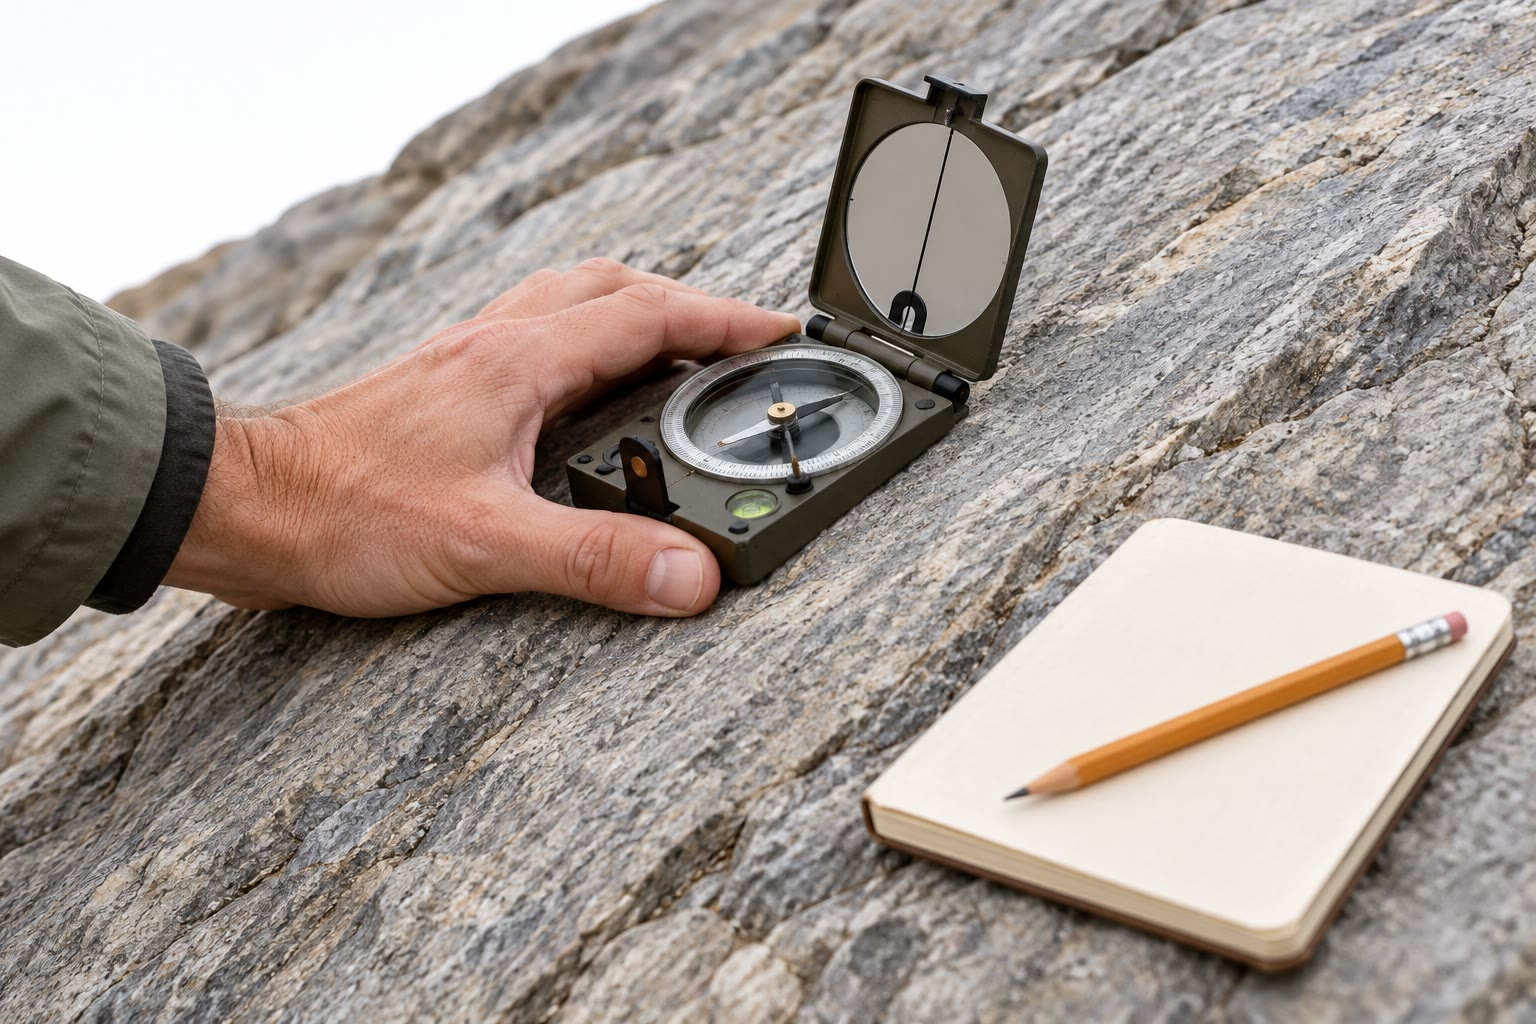
\includegraphics[width=\linewidth]{images/book5/ai/b3-compass-clinometer.jpg}

{\scriptsize Une boussole-clinomètre posée contre une surface rocheuse inclinée, avec un
carnet de terrain. Illustration générée par IA.}
\end{minipage}
\end{inthefield}

\section{Exercices}

\begin{exercise}[$\star$]\label{exo:b3:structural-analysis:1}
Donner l'azimut et le plongement du \omterm{def:b3:structural-analysis:stereo}{pôle} du plan $040/30$ (sens du pendage,
pendage). Donner l'attitude du plan dont le \omterm{def:b3:structural-analysis:stereo}{pôle} a pour azimut \ang{315} et plonge
de \ang{20}.
\end{exercise}

\begin{exercise}[$\star$]\label{exo:b3:structural-analysis:2}
Une droite plonge de \ang{30}. À quelle distance du centre se place-t-elle sur
un \omterm{def:b3:structural-analysis:stereo}{canevas équiangle} et sur un canevas équivalent, tous deux de rayon \qty{10}{cm}~?
\end{exercise}

\begin{exercise}[$\star$]\label{exo:b3:structural-analysis:3}
Les flancs d'un pli ont pour attitudes $090/30$ et $270/30$. Calculer
l'angle entre leurs \omterm{def:b3:structural-analysis:stereo}{pôles} par le produit scalaire des normales, l'angle entre flancs,
et la classe du pli.
\end{exercise}

\begin{exercise}[$\star$]\label{exo:b3:structural-analysis:4}
Une faille $090/60$ porte des stries de pitch \ang{-45}. Avec le vecteur direction
$\vec s = (0, 1, 0)$ et le vecteur de plus grande pente $\vec d$ du plan, le glissement
du toit est $\vec u = \cos r\,\vec s - \sin r\,\vec d$. Calculer
$\vec d$, $\vec u$, ainsi que l'azimut et le plongement du glissement. Nommer la faille.
\end{exercise}

\begin{exercise}[$\star\star$]\label{exo:b3:structural-analysis:5}
Les flancs d'un pli ont pour attitudes $060/40$ et $250/30$. Calculer l'azimut
et le plongement de son axe, ainsi que son angle entre flancs.
\end{exercise}

\begin{exercise}[$\star\star$]\label{exo:b3:structural-analysis:6}
Calculer la fraction de la surface du canevas située à l'intérieur du cercle des
droites plongeant de plus de \ang{60}, sur le canevas équivalent et sur le \omterm{def:b3:structural-analysis:stereo}{canevas
équiangle}, ainsi que la fraction des directions de l'hémisphère inférieur qui plongent
de plus de \ang{60}. Quel canevas faut-il utiliser pour compter les \omterm{def:b3:structural-analysis:stereo}{pôles}~?
\end{exercise}

\begin{exercise}[$\star\star$]\label{exo:b3:structural-analysis:7}
Trois \omterm{def:b3:structural-analysis:stereo}{pôles} se trouvent dans le plan vertical est--ouest, à \ang{-20}, $0$ et
\ang{20} de la verticale~: $\vec p = (\sin a, 0, -\cos a)$. Calculer leur \omterm{def:b3:structural-analysis:orientation-tensor}{tenseur
d'orientation}, ses valeurs propres et vecteurs propres, et l'\omterm{def:b3:structural-analysis:pi}{axe bêta}. Pourquoi
la plus petite valeur propre est-elle exactement nulle~?
\end{exercise}

\begin{exercise}[$\star\star$]\label{exo:b3:structural-analysis:8}
Placer sur le diagramme de Flinn l'ellipsoïde $X : Y : Z = 3 : 1.5 : 1$, puis l'ellipsoïde
à volume constant avec $X = 1.8$ et $Y = 1.1$. Calculer $k$ pour
chacun et nommer la déformation.
\end{exercise}

\begin{exercise}[$\star\star$]\label{exo:b3:structural-analysis:9}
Dans une coupe parallèle à l'étirement, des ooïdes initialement circulaires sont
des ellipses de rapport d'axes $2.25$, toutes parallèles, et l'aire de chacune est
inchangée. Calculer les étirements principaux et l'extension selon le grand
axe. Avant la déformation, les centres des ooïdes n'étaient jamais plus proches que
\qty{0.4}{mm}~: donner les demi-axes du vide du diagramme de Fry.
\end{exercise}

\begin{exercise}[$\star\star\star$]\label{exo:b3:structural-analysis:10}
À $\theta = \ang{60}$ du nadir, calculer l'étirement selon le rayon,
$\mathrm dr/(R\,\mathrm d\theta)$, et autour du cercle, $r/(R\sin\theta)$,
pour les deux projections. Vérifier le théorème sur les projections, et donner le rapport
des axes de l'ovale dans lequel le canevas équivalent transforme un très petit
cercle à cet endroit.
\end{exercise}

\begin{exercise}[$\star\star\star$]\label{exo:b3:structural-analysis:11}
Dans un régime décrochant, $\sigma_1$ est horizontale vers \ang{000},
$\sigma_3$ horizontale vers \ang{090} et $\sigma_2$ verticale. Une faille verticale
de direction \ang{020}. Sans calculer $\vec\tau$, montrer que son glissement est
horizontal pour tout $\Phi$. Calculer ensuite $-\vec\tau$ pour $\Phi = 0.4$ avec
la normale au plan $\vec n = (\cos\ang{20}, -\sin\ang{20}, 0)$ et donner le
sens du glissement.
\end{exercise}

\begin{exercise}[$\star\star\star$]\label{exo:b3:structural-analysis:12}
Une coupe de \qty{20}{km} de long traverse un train de plis de décollement. Deux horizons
distants de \qty{1.0}{km}, se trouvent au-dessus de leur niveau initial d'une aire
de \qty{6.0}{km^2} (inférieur) et \qty{7.5}{km^2} (supérieur). Calculer le raccourcissement,
la profondeur du décollement sous l'horizon inférieur, la longueur initiale de la
coupe et sa variation relative de longueur.
\end{exercise}

\section{Problème~: plis et failles des collines de Varden}

\begin{problem}[{Problème du week-end --- l'axe d'un pli, la contrainte
d'un système de failles et la restauration d'une coupe, dans une région fictive}]
\label{pb:b3:structural-analysis:1}
% values: calc/ch08.py; figdata/bachelor-3/stereonet.py (data invented from region.py)
Dans les collines de Varden, région fictive de la série, une couverture mésozoïque repose sur un
socle de schistes et de granite. La couverture est plissée en un anticlinal droit
et un synclinal droit à flancs rectilignes, puis recoupée par une faille normale. Un
géologue a mesuré douze plans de stratification sur les deux flancs de l'anticlinal
(sens du pendage/pendage, en degrés)~:

\begin{center}
\small
\begin{tabular}{l|cccccc}
\hline
flanc est & 075/13 & 084/11 & 089/13 & 079/14 & 086/12 & 072/11 \\
flanc ouest & 283/11 & 272/13 & 281/14 & 288/10 & 276/13 & 274/12 \\
\hline
\end{tabular}
\end{center}

Les sommes des normales unitaires ascendantes des six mesures de chaque flanc sont
$\vec S_E = (1.2583, 0.2017, 5.8604)$ et $\vec S_W = (-1.2445, 0.1886,
5.8636)$ (est, nord, haut). Cinq failles portent des stries (sens du pendage/pendage,
pitch du glissement du toit)~: $120/60/{-90}$ (la faille principale), $150/55/{-76}$,
$090/65/{-108}$, $200/70/{-78}$ et $060/50/{-105}$. La faille principale présente un
rejet vertical de \qty{200}{m}. Les axes de l'anticlinal et du synclinal sont distants
de \qty{4}{km}, de sorte que les plis se répètent tous les \qty{8}{km} d'est en ouest.

\medskip\noindent\textbf{Partie I --- Pôles et axe bêta.}
\begin{enumerate}
  \item Donner l'azimut et le plongement du \omterm{def:b3:structural-analysis:stereo}{pôle} de la mesure $075/13$, ainsi que
        sa distance au centre d'un canevas équivalent de rayon
        \qty{10}{cm}.
  \item Calculer la normale unitaire ascendante de la mesure $075/13$~; la comparer
        à $\vec S_E$ en module.
  \item Calculer l'attitude moyenne de chaque flanc à partir de $\vec S_E$ et $\vec S_W$,
        les longueurs des résultantes moyennes, et l'écart quadratique moyen des
        mesures autour de leurs moyennes.
  \item Calculer $\vec S_E\times\vec S_W$, ainsi que l'azimut et le plongement
        de l'\omterm{def:b3:structural-analysis:pi}{axe bêta}.
  \item Calculer l'angle entre les deux normales moyennes, l'angle entre flancs,
        et la classe du pli.
  \item Le plan axial de ce pli symétrique contient l'\omterm{def:b3:structural-analysis:pi}{axe bêta} et est
        perpendiculaire à $\vec m_E - \vec m_W$, la différence des normales unitaires
        moyennes. Donner son attitude~; le pli est-il droit~?
  \item Donner l'attitude de la ceinture $\pi$, et expliquer pourquoi les \omterm{def:b3:structural-analysis:stereo}{pôles} se trouvent
        sur elle.
\end{enumerate}

\medskip\noindent\textbf{Partie II --- Le tenseur d'orientation.}
Le \omterm{def:b3:structural-analysis:orientation-tensor}{tenseur d'orientation} des douze \omterm{def:b3:structural-analysis:stereo}{pôles} est
\[
  T = \begin{pmatrix} 0.04400 & 0.00035 & 0.00109\\ 0.00035 & 0.00144 & 0.03179\\
  0.00109 & 0.03179 & 0.95456 \end{pmatrix},
\]
avec les valeurs propres $0.95562$, $0.04400$ et $0.00038$.
\begin{enumerate}[resume]
  \item Vérifier que la trace de $T$ vaut 1. Avec $\vec b = (0.0053, -0.9994,
        0.0333)$, le vecteur unitaire selon $\vec S_E\times\vec S_W$, calculer
        $\vec b^{\mathsf T}T\vec b$. Que dit le résultat de $\vec b$~?
  \item Calculer l'écart angulaire quadratique moyen entre les \omterm{def:b3:structural-analysis:stereo}{pôles} et la ceinture.
  \item Expliquer la valeur de $\lambda_2$ à partir des pendages des flancs.
  \item Le pli est-il cylindrique à la précision des mesures près~?
  \item Le plongement de l'\omterm{def:b3:structural-analysis:pi}{axe bêta} est fixé par l'inclinaison nord--sud de la
        ceinture, à laquelle chaque \omterm{def:b3:structural-analysis:stereo}{pôle} contribue avec la dispersion trouvée à
        la question~9. Estimer l'erreur type du plongement.
\end{enumerate}

\medskip\noindent\textbf{Partie III --- La paléocontrainte.}
\begin{enumerate}[resume]
  \item De quel type est la faille principale~? Selon Anderson, donner les
        directions de $\sigma_1$, $\sigma_2$ et $\sigma_3$.
  \item Montrer, à l'aide du théorème sur la direction de glissement, que la faille principale
        glisse droit selon son pendage pour toute valeur de $\Phi$. Que
        nous apprend-elle sur $\Phi$~?
  \item Pour la faille $150/55$, calculer $\vec n$ et ses composantes $n_1 =
        \vec n\cdot\vec e_1$ et $n_2 = \vec n\cdot\vec e_2$, avec $\vec e_1$
        vertical et $\vec e_2$ horizontal, dirigé vers \ang{030}.
  \item Son glissement donne $\vec w = \vec n\times\vec u = (0.771, 0.605, 0.198)$.
        Calculer $\Phi$.
  \item Les trois autres petites failles donnent $\Phi = 0.294$, $0.301$ et
        $0.306$. Donner la moyenne, et dire d'où provient la dispersion.
  \item Que dit $\Phi = 0.3$ de $\sigma_2$~?
  \item Calculer les axes P et T de la faille principale (à \ang{45} du
        plan, dans son plan de pendage), et les comparer à $\sigma_1$ et
        $\sigma_3$.
\end{enumerate}

\medskip\noindent\textbf{Partie IV --- Restauration d'une coupe est--ouest.}
\begin{enumerate}[resume]
  \item Calculer le pendage apparent du flanc est, $080.9/12.3$, sur une
        coupe est--ouest.
  \item En prenant les flancs à \ang{12} sur la coupe, calculer la longueur restaurée
        d'une longueur d'onde de pli, le raccourcissement et la variation relative
        de longueur.
  \item Calculer la hauteur de la crête de l'anticlinal au-dessus des synclinaux et
        l'aire en excès d'une longueur d'onde, en supposant que les synclinaux sont restés à
        leur niveau initial.
  \item Calculer la profondeur du décollement sous l'horizon plissé. Les plis peuvent-ils
        être décollés à la base de la couverture, à quelques centaines de mètres
        de profondeur~?
  \item Calculer le rejet horizontal et le glissement de la faille principale sur une coupe orientée
        à \ang{120}.
  \item Sur la coupe est--ouest, calculer le pendage apparent de la faille et
        son rejet horizontal apparent. Quelle coupe doit être restaurée~?
  \item Dans quel ordre la faille et les plis sont-ils restaurés, et où sont placées les
        \omterm{def:b3:structural-analysis:restoration}{lignes de référence}~?
  \item Quel est le plongement de l'axe du pli de Varden, déduit des douze
        mesures~?
\end{enumerate}
\end{problem}
